% Author: Adolfo Centeno 
% Kubeet Corp
% www.kubeet.com

 
\documentclass{beamer}
\setbeamertemplate{navigation symbols}{}
\usepackage[utf8]{inputenc}
\usepackage{beamerthemeshadow}
\usepackage{listings}

\begin{document}
\title{IoTEC}  
\author{Adolfo Centeno, Daniel Perez, Fabio Galo}
\date{\today} 

\begin{frame}
\titlepage
\end{frame}

\begin{frame}\frametitle{Table of contents}\tableofcontents
\end{frame} 


\section{Introduction} 

\begin{frame}\frametitle{Internet of things} 


\begin{figure}
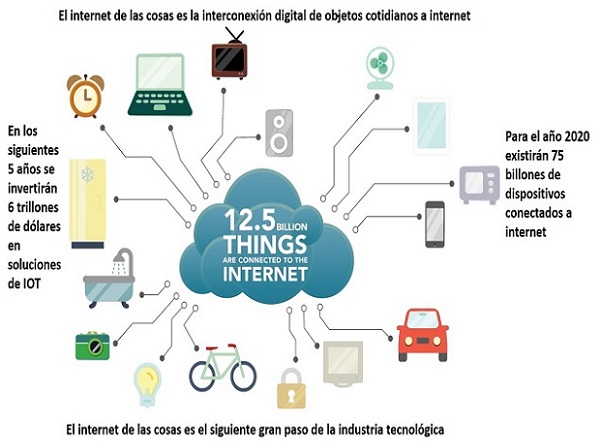
\includegraphics[scale=0.9]{iot} 
\end{figure}




\end{frame}

\begin{frame}\frametitle{IoTEC - RoadMap} 
\begin{figure}
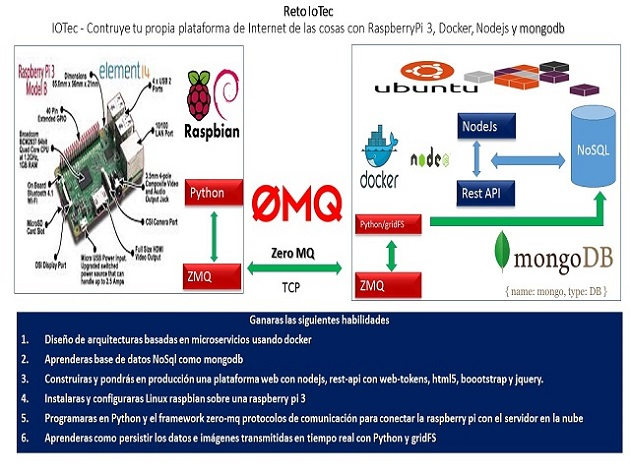
\includegraphics[scale=0.6]{iotec_roadmap} 
\end{figure}




\end{frame}


 
\begin{frame}\frametitle{IOTEC - Schedule} 

\begin{itemize}
\item Day 1 (Introduction, Google Compute Engine Client and Mongodb database)   
\item Day 2 (Docker, Nodejs) 
\item Day 3 (Raspbian install, python, zero-mq) 
\item Day 4 (Programming sockets with python/zero-mq)
\item Day 5 (Final project)
\end{itemize} 

\end{frame}

\section{Install, Google Compute Engine Client} 
\begin{frame}\frametitle{The cloud computing stack – SaaS, PaaS, and IaaS} 

We can represent cloud computing as a stack of three different categories:
\begin{itemize}
\item Software as a Service (SaaS)   
\item Platform as a Service (PaaS) 
\item Infrastructure as a Service (IaaS)
 

\end{itemize} 



\end{frame}

\subsection{Google App Engine (GAE)}
\begin{frame} 

Hosting + Compute 

There are two options if we want to host an application on Google Cloud Platform:



\begin{enumerate}

\item
Google App Engine: This is Google's PaaS and it will not be covered in this project.

\item
Google Compute Engine: This is Google's IaaS and lets users run virtual
machines on Google's infrastructure with a variety of hardware and
software configurations.
\end{enumerate}

\end{frame}


\subsection{Instalación de GCE Client (I)}


\defverbatim[colored]\lstA{
 \begin{lstlisting}[language=bash,showstringspaces=false, basicstyle={\tiny}, keywordstyle=\color{red}]
export CLOUD_SDK_REPO="cloud-sdk-$(lsb_release -c -s)"
 \end{lstlisting}
}


\defverbatim[colored]\lstB{
 \begin{lstlisting}[language=bash,showstringspaces=false, basicstyle={\tiny}, keywordstyle=\color{red}]
echo "deb http://packages.cloud.google.com/apt $CLOUD_SDK_REPO main" | 
     sudo tee -a /etc/apt/sources.list.d/google-cloud-sdk.list
 \end{lstlisting}
}

\defverbatim[colored]\lstC{
 \begin{lstlisting}[language=bash,showstringspaces=false, basicstyle={\tiny}, keywordstyle=\color{red}]
curl https://packages.cloud.google.com/apt/doc/apt-key.gpg | sudo apt-key add -
 \end{lstlisting}
}

\begin{frame} 

Ubuntu/Debian install (Part I)

\begin{block}{Create an environment variable for the correct distribution}
\lstA
\end{block}


\begin{block}{Add the Cloud SDK distribution URI as a package source:}
\lstB
\end{block}

\begin{block}{Import the Google Cloud public key:}
\lstC
\end{block}


	
\end{frame}


\subsection{Instalación de GAE (II)}

\defverbatim[colored]\lstD{
 \begin{lstlisting}[language=bash,showstringspaces=false, basicstyle={\tiny}, keywordstyle=\color{red}]
sudo apt-get update && sudo apt-get install google-cloud-sdk
 \end{lstlisting}
}


\defverbatim[colored]\lstE{
 \begin{lstlisting}[language=bash,showstringspaces=false, basicstyle={\tiny}, keywordstyle=\color{red}]
sudo apt-get install google-cloud-sdk-app-engine-python
 \end{lstlisting}
}

\defverbatim[colored]\lstauthlogin{
 \begin{lstlisting}[language=bash,showstringspaces=false, basicstyle={\tiny}, keywordstyle=\color{red}]

$ sudo gcloud auth login  # login to Google 

NOTE: 
gmail user : mindlesssmile72@gmail.com
password   : semanai2017

 \end{lstlisting}
}

\defverbatim[colored]\lstnewuser{
 \begin{lstlisting}[language=bash,showstringspaces=false, basicstyle={\tiny}, keywordstyle=\color{red}]

$ sudo adduser [username]           # add user
$ sudo usermod -aG sudo [username]  # grant root privileges
$ su [username]                     # swith user to [username]  
$ whoami                            # display current user
$ cd ~                              # change directory to user's home
$ pwd                               # display path working directory

 \end{lstlisting}
}



\defverbatim[colored]\lstconnect{
 \begin{lstlisting}[language=bash,showstringspaces=false, basicstyle={\tiny}, keywordstyle=\color{red}]
# set the default project 
$ sudo gcloud config set project adsoft-iosclient  

# print virtual private servers
$ sudo gcloud compute instances list  

# check network connectivity
$ ping 35.185.213.109                 

# login with secure shell (ssh) to compute instance with [username]
$ sudo gcloud compute ssh [username]@mindlesssmile72 --zone us-west1-b

# show home directory
$ ls /home 

 \end{lstlisting}
}

\begin{frame} 

Ubuntu/Debian install  (Part II)

\begin{block}{Update and install the Cloud SDK:}
\lstD
\end{block}


\begin{block}{Install the additional component:}
\lstE
\end{block}



	
\end{frame}




\begin{frame} 

Ubuntu/Create new user

\begin{block}{add new user}
\lstnewuser
\end{block}

\begin{block}{Run gcloud auth login to get started:}
\lstauthlogin
\end{block}
	
\end{frame}



\begin{frame} 

Connect to Google Compute Engine

\begin{block}{Set project/connect with ssh to GCE}
\lstconnect
\end{block}

	
\end{frame}



\section{MongoDB} 
\begin{frame}\frametitle{MongoDB - Overview} 

What's MongoDB

\begin{itemize}

\item MongoDB is a document database with the scalability and flexibility
 
\item MongoDB stores data in flexible, JSON-like documents

\item MongoDB is free and open-source

\item TCP port: 27017 

\item MongoDB connection:  mongodb://35.185.213.109:27017/ourdatabase 


\end{itemize} 

\end{frame}


\subsection{MongoDB - Connect}

\defverbatim[colored]\lstmongoconnect{
 \begin{lstlisting}[language=bash,showstringspaces=false, basicstyle={\tiny}, keywordstyle=\color{red}]
# start mongodb
$ sudo service mongod start

# start mongodb
$ sudo service mongod status

# connect to mongo
$ mongo localhost   # other example:  mongo 35.185.213.109:27017

$ show databases;

# exit from mongo shell
$ exit

 \end{lstlisting}
}



\defverbatim[colored]\lstmongocreatedb{
 \begin{lstlisting}[language=bash,showstringspaces=false, basicstyle={\tiny}, keywordstyle=\color{red}]
# show databases
> show dbs

# create database
> user iotec-[username] 

# create device collection
> db.devices.insert({"name":"edison"})

$ show collections;
> show collections

# show devices
$ db.devices.find()

 \end{lstlisting}
}



\defverbatim[colored]\lstmongocreate{
 \begin{lstlisting}[language=bash,showstringspaces=false, basicstyle={\tiny}, keywordstyle=\color{red}]

# create one
> db.devices.insertOne({"name":"lego mindstorm ev3"})

# create many
> db.devices.insertMany([{"name":"arduino one"}, {"name": "arduino mega"}])

# list all devices
> db.devices.find()

 \end{lstlisting}
}



\defverbatim[colored]\lstmongoread{
 \begin{lstlisting}[language=bash,showstringspaces=false, basicstyle={\tiny}, keywordstyle=\color{red}]

# query filter 
> db.devices.find({"name":"edison"})

# contains query filter
> db.devices.find({name: /^arduino/})

# list top n devices
> db.devices.find().limit(3)

# in
> db.devices.find( { name : { $in: [ "edison", "arduino one" ] } } )


# and 
> db.devices.find({_id: ObjectId("59c8975c95b0585b53e4b728")}, {name: /^arduino/})

# or
> db.devices.find({$or: [{name: "intel edison"}, {name: "dron pxfmini"}]});

 \end{lstlisting}
}




\defverbatim[colored]\lstmongoupdate{
 \begin{lstlisting}[language=bash,showstringspaces=false, basicstyle={\tiny}, keywordstyle=\color{red}]

# update one document
> db.devices.updateOne({"name":"intel edison"}, {$set: {name: "edison"}})
> db.devices.find()

# update many documents
> db.devices.updateMany({"name": /^arduino/}, {$set: {name: "arduino"}})
> db.devices.find()


# update one document using update operator (update the first document)
> db.devices.update({"name":"arduino"}, {$set: {name: "arduino one"}})
> db.devices.find()

# update many documents, using update operator (multiples update)
> db.devices.update({"name": /^arduino/}, {$set: {name: "arduino"}}, {multi : true})
> db.devices.find()



 \end{lstlisting}
}


\defverbatim[colored]\lstmongodelete{
 \begin{lstlisting}[language=bash,showstringspaces=false, basicstyle={\tiny}, keywordstyle=\color{red}]

# delete one document
> db.devices.deleteOne({"name":"edison"})
> db.devices.find()

# delete many documents
> db.devices.deleteMany({"name": /^arduino/})
> db.devices.find()

# delete one document wirh remove operator
> db.devices.remove({"name": /^lego/}, 1)
> db.devices.find()

# delete many documents with remove operator
> db.devices.remove({"name": /^dron/})
> db.devices.find()




 \end{lstlisting}
}


\begin{frame} 

\begin{block}{Start/Stop/Status/Restart mongo}
\lstmongoconnect
\end{block}


\end{frame}


\subsection{MongoDB - Create database/show collections}
\begin{frame} 

\begin{block}{Create database}
\lstmongocreatedb
\end{block}

\end{frame}


\subsection{Create, Read, Update, Delete}
\begin{frame}{Create} 

\begin{block}{Create documents}
\lstmongocreate
\end{block}

\end{frame}


\begin{frame}{Read} 

\begin{block}{Query documents}
\lstmongoread
\end{block}

\end{frame}


\begin{frame}{Update} 

\begin{block}{Update documents}
\lstmongoupdate
\end{block}

\end{frame}



\begin{frame}{Delete} 

\begin{block}{Delete documents}
\lstmongodelete
\end{block}

\end{frame}

\end{document}
